\documentclass{ifacconf}

\usepackage{natbib}            % you should have natbib.sty
\usepackage{graphicx}          % Include this line if your 
                               % document contains figures,
%\usepackage[dvips]{epsfig}    % or this line, depending on which
                               % you prefer.
\usepackage[utf8]{inputenc} % ��� pakken
\usepackage[T1]{fontenc}
% predefined environments
%\begin{thm} ... \end{thm}		% Theorem
%\begin{lem} ... \end{lem}		% Lemma
%\begin{claim} ... \end{claim}	% Claim
%\begin{conj} ... \end{conj}	% Conjecture
%\begin{cor} ... \end{cor}		% Corollary
%\begin{fact} ... \end{fact}	% Fact
%\begin{hypo} ... \end{hypo}	% Hypothesis
%\begin{prop} ... \end{prop}	% Proposition
%\begin{crit} ... \end{crit}	% Criterion


\begin{document}

\begin{frontmatter}

\title{Centralized State Estimation of Distributed Maritime Autonomous Surface Oceanographers\thanksref{footnoteinfo}} % Title, preferably not more than 10 words.

\thanks[footnoteinfo]{This work was supported in part by the National Technological Agency. (sponsor and financial support acknowledgment goes here). Paper titles should be written in uppercase and lowercase letters, not all uppercase.}

\author[First]{Rasmus L. Christensen} 
\author[First]{Frederik Juul} 
\author[First]{Nick \O stergaard}
\author[First]{Attila Fodor}
\author[First]{Tudor Muresan}
\address[First]{Department of Electronic Systems, Aalborg University, Fredrik Bajers Vej 7, 9220 Aalborg \O st, Denmark (e-mail: \{ralch,nickoe,fjuul,tudor,attila\}@es.aau.dk)}                                            
          
%\begin{keyword}                           % Five to ten keywords,  
%Cicero; Catiline; orations.               % chosen from the IFAC 
%\end{keyword}                             % keyword list or with the 
                                          % help of the Automatica 
                                          % keyword wizard


\begin{abstract}                          % Abstract of not more than 250 words.
This paper considers the subject of running a centralized controller for the purpose of navigating a small Autonomous Surface Vehicle (ASV). The centralized controller is using a Kalman filter as a state predictor to improve the precision of the navigational aids mounted aboard. The work presents the design of the motion control system as well as the development of a protocol used to push through as much data on a standard 9.6 kbps data link simplex link.

The performance for the algorithms developed in this project, have been tested in Limfjorden in Aalborg, and towards the end, results of these tests are shown. 
\end{abstract}

\end{frontmatter}

\section{Introduction}
As up to date mapping of the coastal areas around Greenland is not available, and the process of creating these are a both time consuming and expensive task. One way to reduce both the costs and the amount of time invested in such a project could be to develop small autonomous drones to carry out this task. 

These drones should be controlled by a mothership, which would utilize a simple data link, both to preserve bandwith, but also to make the duration at which the ships are able to sail as long as possible, by limiting the power consumption. 

Currently the main focus of autonomous vehicles have been on aerial, ground and underwater vehicles, why there is close to no research going on about small autonomous surface vessels. An example of such a vessel is the Stingray ASV developed by Isreali Based Elbit Systems. The purpose of this vehicle is somewhat military related, where the purpose of measuring the coastal areas around Greenland are purely humanitarian,

{\bf Do not change the font sizes or line spacing to squeeze more text into a limited number of pages. Use italics for emphasis; do not underline}.

\subsection{Problem statement}
\begin{hypo} Is it possible to develop a centralized state estimator for use in the maritime environment using a small data link \end{hypo}

\subsection{A subsection}
Bifurcation: Plot of local maxima of $x$ with damping $a$ decreasing (Fig.~\ref{fig1}).

To insert images in Word, position the cursor at the insertion point and either use Insert | Picture | From File or copy the image to the Windows clipboard and then Edit | Paste Special | Picture (with �Float over text� unchecked). 

IFAC will not do any final formatting of your paper. Your manuscript should be �camera-ready.� Page limits vary from conference to conference. Please observe the conference page limits of the conference for which your paper is intended. {\bf Please do not modify margins. If you are creating a document on your own, please observe the margins as listed in Table 1}.

\begin{figure}
	\begin{center}
		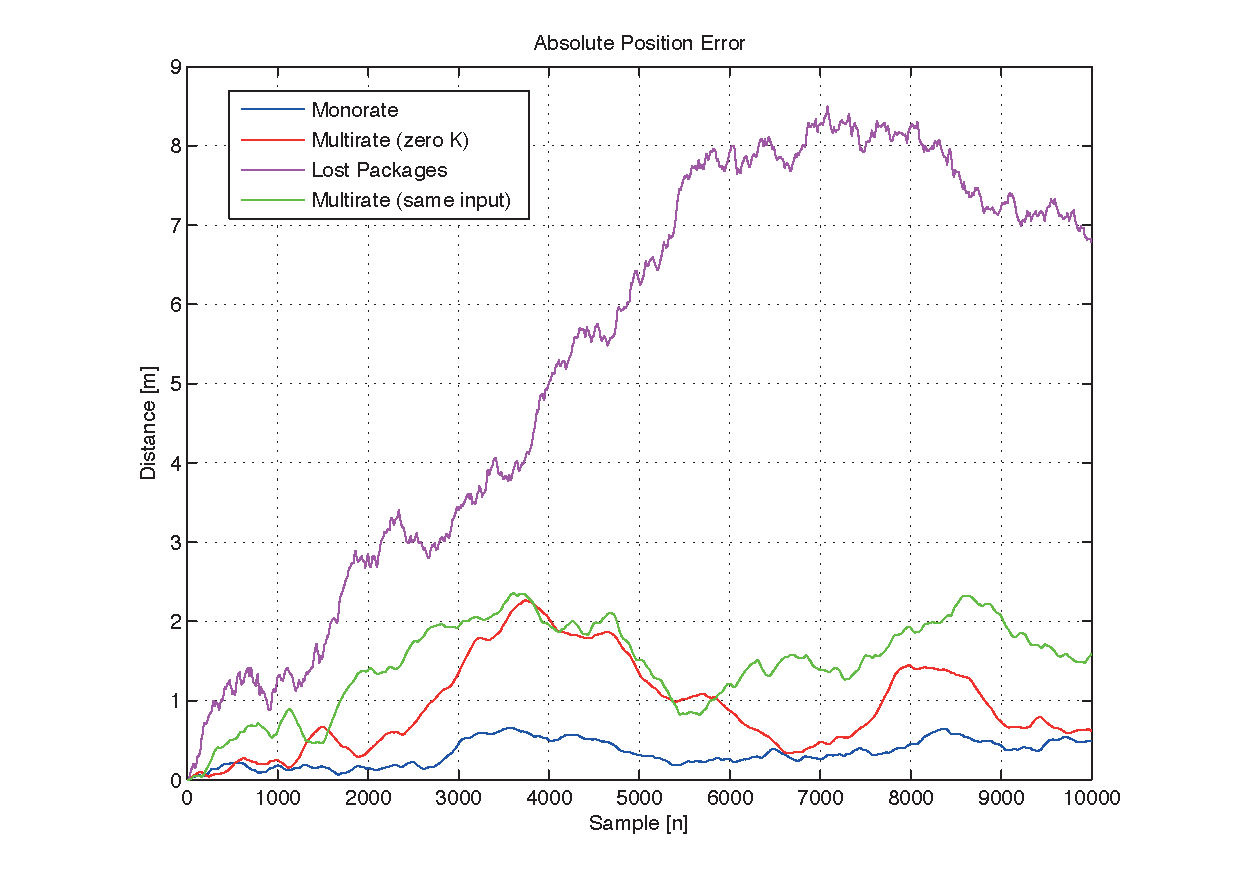
\includegraphics[height=6cm]{img/10percent}    % The printed column  
		\caption{Bifurcation: Plot of local maxima of $x$ with damping $a$ decreasing}  % 			width is 8.4 cm.
		\label{fig1}                                 % Size the figures 
	\end{center}                                 % accordingly.
\end{figure}

\section{Methods}

The methods developed in this project - and the papers. 2

\subsection{Path planning algorithm}

{\bf Please use this document as a �template� to prepare your manuscript. For submission guidelines, follow instructions on paper submission system as well as the Conference website.}

Note that conferences impose strict page limits, so it will be better for you to prepare your initial submission in the camera ready layout so that you will have a good estimate for the paper length. Additionally, the effort required for final submission will be minimal.

Some words might be appropriate describing equation~(\ref{e1}), if 
we had but time and space enough.
\begin{equation} \label{e1}
{{\partial F}\over {\partial t}} =
D{{\partial^2 F}\over {\partial x^2}}.
\end{equation}
See \cite{Abl:56}, \cite{AbTaRu:54}, \cite{Keo:58} and \cite{Pow:85}.

\subsubsection{Control algorithm}
This equation goes far beyond the celebrated theorem ascribed to the great Pythagoras by his followers.
\begin{thm}
The square of the length of the hypotenuse of a right triangle equals the sum of the squares 
of the lengths of the other two sides.
\end{thm}
\begin{pf}
The square of the length of the hypotenuse of a right triangle equals the sum of the squares 
of the lengths of the other two sides.
\end{pf}


\section{Math}

If you are using Word, use either the Microsoft Equation 
Editor or the MathType add-on for equations in your paper (Insert | Object | Create New | Microsoft Equation or MathType Equation). �Float over text� should not be selected. Of course LaTeX manages equations through built-in macros.

\section{Units}

\section{Results}

\subsection{Control verification}

Verification of the controllers.

\subsection{Path planning results}

Results of the path planning algorithm

\subsection{Kalman filtering verification}

Combined test of the controller and the path planner.

\subsection{Combined test}

Something about the packet loss. 

\subsection{Other tests}

Something else?


\section{Conclusion}

A conclusion section is not required. Although a conclusion may review the main points of the paper, do not replicate the abstract as the conclusion. A conclusion might elaborate on the importance of the work or suggest applications and extensions. 

\begin{ack}                               % Place acknowledgements
A special thank should be given to Assistant Professor Carles Navarro Manch�n, Section for Navigation and Communication, Department of Electronic Systems, Aalborg University for his help with tuning the Kalman filter.  % here.
\end{ack}

%\bibliographystyle{alpha}        % Include this if you use bibtex 
%\bibliography{autosam}           % and a bib file to produce the 
%\bibliography{autosam}
                                 % bibliography (preferred). The
                                 % correct style is generated by
                                 % Elsevier at the time of printing.

\begin{thebibliography}{xx}

\bibitem[Able(1956)]{Abl:56}
B.C. Able.
\newblock Nucleic acid content of microscope.
\newblock \emph{Nature}, 135:\penalty0 7--9, 1956.

\bibitem[Able et~al.(1954)Able, Tagg, and Rush]{AbTaRu:54}
B.C. Able, R.A. Tagg, and M.~Rush.
\newblock Enzyme-catalyzed cellular transanimations.
\newblock In A.F. Round, editor, \emph{Advances in Enzymology}, volume~2, pages
  125--247. Academic Press, New York, 3rd edition, 1954.

\bibitem[Keohane(1958)]{Keo:58}
R.~Keohane.
\newblock \emph{Power and Interdependence: World Politics in Transitions}.
\newblock Little, Brown \& Co., Boston, 1958.

\bibitem[Powers(1985)]{Pow:85}
T.~Powers.
\newblock Is there a way out?
\newblock \emph{Harpers}, pages 35--47, June 1985.

\bibitem[Soukhanov(1992)]{Heritage:92}
A.~H. Soukhanov, editor.
\newblock \emph{{The American Heritage. Dictionary of the American Language}}.
\newblock Houghton Mifflin Company, 1992.

\end{thebibliography}








\appendix
\section{A summary of Latin grammar}    % Each appendix must have a short title.
\section{Some Latin vocabulary}         % Sections and subsections are supported  
                                        % in the appendices.
\end{document}